%
% CHAPTER 7.- Interesting Questions
%

\chapterimage{thinker.pdf}

\chapter{Interesting Questions}
\label{chap:Interesting-Research-Questions}

\begin{quote}
\begin{flushright}
\emph{It is not the answer that enlightens,\\
but the question. \\}
Eugène Ionesco
\end{flushright}
\end{quote}
\bigskip

In this chapter, we introduce a set of metrics for classifying research topics according to their potential to generate interesting problems, along with a methodology for the assisted discovery of new research questions. The objective is to propose new directions, novel research ideas, that contribute to reducing nescience, that is, to diminishing the extent of the scientific unknown. The proposed methodology supports both the identification of new applications for existing tools to address open problems (the known unknown\index{Known unknown}) and the discovery of entirely new and previously unexplored research directions (the unknown unknown\index{Unknown unknown}). While the methodology is applicable to both intradisciplinary and interdisciplinary topics, the most impactful results typically arise in the latter case. In Chapter \ref{chap:computational-creativity}, we demonstrate the methodology in practice and propose several new questions and research topics.

We have already examined three dimensions for classifying research topics: miscoding (Chapter \ref{chap:Miscoding}), inaccuracy (Chapter \ref{chap:Error}), and surfeit (Chapter \ref{chap:Redundancy}). These metrics allow us to quantitatively assess our level of understanding of a topic, a concept we refer to as nescience. In this section, we introduce two additional metrics for characterizing topics: relevance (Section \ref{sec:relevance}) and applicability (Section \ref{sec:applicability}). Relevance measures the impact a topic has on people's lives and complements the existing metrics of nescience. Applicability quantifies how frequently a topic has been applied in other domains and helps identify new uses for existing technologies.

What is proposed in this chapter is an algebraic approach to the assisted discovery of potentially interesting research questions, grounded in the theory of nescience. The objective of this methodology is twofold. On the one hand, it aims to support researchers in their day-to-day work. The methodology can be used to uncover novel tools that may be applied to a given problem, or to identify new problems where existing tools could be effectively used. In its more advanced form, the methodology facilitates the exploration of the unknown unknown, that is, research areas that have not yet been conceptualized, described, or even imagined.

On the other hand, because the methodology is based on well-defined mathematical principles, it lends itself to automation. This opens the door for artificial intelligence systems to move beyond their current limitations, namely, their inability to autonomously generate truly novel research directions. By formalizing the process of question discovery, the methodology enables AI to propose interesting and previously unexplored research questions, and even to discover entirely new topics of scientific inquiry.

%
% Relevance
%

\section{Relevance}
\label{sec:relevance}

In this chapter, we propose additional metrics to complement nescience in the task of evaluating the interest of research topics. These metrics will be useful not only for classifying individual topics, but also for developing a methodology for discovering potential solutions to open problems (Section \ref{sec:intro_interesting_questions}), as well as for identifying entirely new research topics (Section \ref{sec:New_Research_Topics}).

One of these new metrics is \emph{relevance}. Relevance quantifies the impact that a research topic has on people's lives. Intuitively, the greater the relevance of a topic, the higher its potential as a source of interesting problems, since it concerns issues that affect many individuals directly.

Before we can measure the relevance of a topic, that is, its impact on people's lives, we must introduce the concept of a \emph{relevance graph}. The relevance graph (see Figure \ref{fig:Relevance-Graph}) captures the relationship between people and the research topics that affect them.

\begin{definition}\index{Relevance Graph}
\label{def:relevance-graph}
We define the \emph{relevance graph}\index{Relevance graph}, denoted by $\mathbf{RG}$, as the bipartite graph $\mathbf{RG} = (\mathcal{T}, \mathcal{P}, E)$, where $\mathcal{T}$ is the set of topics, $\mathcal{P}$ is the set of people, and $E\subseteq\left\{ \left(i,j\right):i\in \mathcal{T},j\in \mathcal{P} \right\}$ is the set of edges between topics and people. An edge $(i, j)$ belong to $E$ if, and only if, person $j$ is affected by topic $i$.
\end{definition}

When we refer to the set of people $\mathcal{P}$, we mean all individuals in the world. A connection between a topic and a person indicates that the person is affected by the topic, not that they are necessarily interested in it. For example, someone researching a cure for diabetes would not be connected to the research topic "diabetes," but someone who actually suffers from the disease would be.

The higher the relevance of a topic, the greater its potential as a source of interesting problems to solve. In this sense, the research topic "how to cure diabetes" is more relevant than "how far dog fleas can jump," because more people are affected by the former than by the latter.

The precise meaning of "\emph{being affected by}" is inherently abstract and must be approximated in practice. For instance, one could argue that the spouse of a person with diabetes is also affected by the disease in some way. In Section \ref{sec:relevance_in_practice}, we will explore how this concept can be operationalized in the context of scientific research topics.

% \begin{figure}[h]
% \centering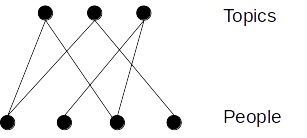
\includegraphics[scale=0.7]{bipartite_graph}
% \caption{\label{fig:Relevance-Graph}Relevance Graph}
% \end{figure}

\begin{figure}[t]
\centering
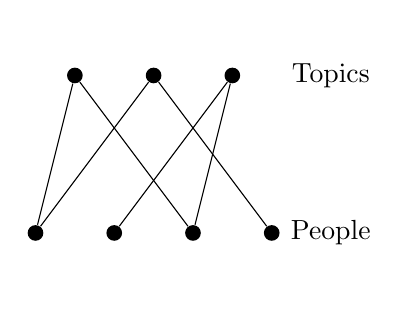
\begin{tikzpicture}[scale=1, every node/.style={circle, fill=black, inner sep=2pt}]

% Nodes: Topics (top row)
\node (t1) at (0.5,2) {};
\node (t2) at (1.5,2) {};
\node (t3) at (2.5,2) {};

% Nodes: People (bottom row)
\node (p1) at (0,0) {};
\node (p2) at (1,0) {};
\node (p3) at (2,0) {};
\node (p4) at (3,0) {};

% Edges
\draw (t1) -- (p1);
\draw (t1) -- (p3);
\draw (t2) -- (p1);
\draw (t2) -- (p4);
\draw (t3) -- (p2);
\draw (t3) -- (p3);

% Labels
\node[draw=none, fill=none] at (3.75,2) {Topics};
\node[draw=none, fill=none] at (3.75,0) {People};

\end{tikzpicture}
\caption{\label{fig:Relevance-Graph}Relevance Graph}
\end{figure}

Optionally, we can assign a weight $w_{ij} \in [0,1]$ to the edges of the graph to indicate the degree to which a person $j$ is affected by a topic $i$. A weight of $1$ could represent a life-or-death dependence, while a weight of $0$ would mean that the person is not affected at all. Figure \ref{fig:Relevance-Graph} shows an example of a relevance graph.

The relevance of a topic measures the extent to which it affects people. This can be assessed either by counting the number of affected individuals or by taking into account the magnitude of the effect.

\begin{definition}\index{Relevance}
\label{def:relevance}
Let $t \in \mathcal{T}$ be a topic, $\mathcal{P}_t \subseteq \mathcal{P}$ the set of people connected to $t$ in the relevance graph, and $w_{tp} \in [0,1]$ the weight of the edge between $t$ and $p \in \mathcal{P}_t$. We define the \emph{relevance} of $t$ as
\[
R(t) = \sum_{p : (t,p) \in E} w_{tp},
\]
\end{definition}

The unweighted relevance $R(t)$ (with $w_{tp} = 1$) counts the number of people affected by the topic, while the weighted relevance $R(t)$ reflects both the number of people and the severity of the effect. A higher relevance value indicates greater potential for generating important and impactful questions.

In practice it is useful to normalize the relevance of a topic so that the least relevant topic has a value of $0$, the most relevant has a value of $1$, and all others lie proportionally in between.

\begin{definition}\index{Normalized relevance}
\label{def:minmax_normalized_relevance}
Let $t \in \mathcal{T}$ be a topic. We define the \emph{min-max normalized relevance} of $t$ as
\[
\bar{R}(t) = \frac{R(t) - \min_{t' \in \mathcal{T}} R(t')}{\max_{t' \in \mathcal{T}} R(t') - \min_{t' \in \mathcal{T}} R(t')}
\]
\end{definition}

This transformation ensures that $\bar{R}(t) \in [0,1]$, with $0$ assigned to the least relevant topic and $1$ to the most relevant. In the degenerate case where all topics have the same relevance, all normalized values are set to $0$.

We could also compute the weighted degree of a person $p$, denoted $R(p)$, defined as the sum of the weights of the edges that link $p$ to topics in the relevance graph. This quantity measures the overall impact of all topics on a particular person. However, this measure is not used in the theory of nescience.

The relation between the weighted relevance of topics and the weighted degrees of people is given by the weighted degree sum formula:
\[
\sum_{t \in \mathcal{T}} R(t) \;=\; \sum_{p \in \mathcal{P}} R(p) \;=\; \sum_{(t,p) \in E} w_{tp}.
\]
In the unweighted case ($w_{tp} = 1$ for all edges), this formula reduces to the standard degree sum formula
\[
\sum_{t \in \mathcal{T}} \deg(t) \;=\; \sum_{p \in \mathcal{P}} \deg(p) \;=\; |E|.
\]

The next proposition shows that, in the weighted case, adding more topics to a research project can only increase its overall relevance. Of course, a research project dealing with "life, the universe, and everything" would be highly relevant, but also highly impractical. How to properly combine research topics will be described in Section \ref{sec:New_Research_Topics}.

\begin{proposition}
Let $S \subseteq \mathcal{T}$ be a finite set of topics and let $t' \in \mathcal{T} \setminus S$ be an additional topic. Then
\[
R(S \cup \{t'\}) \;\geq\; R(S),
\]
where the total weighted relevance of a set of topics $S$ is defined as
\[
R(S) = \sum_{\substack{t \in S \\ p \in \mathcal{P} \\ (t,p) \in E}} w_{tp}.
\]
\end{proposition}
\begin{proof}
We can write
\[
R(S \cup \{t'\}) = \sum_{\substack{t \in S \cup \{t'\} \\ p \in \mathcal{P} \\ (t,p) \in E}} w_{tp}
= R(S) + \sum_{\substack{p \in \mathcal{P} \\ (t',p) \in E}} w_{t'p}.
\]
Since all weights $w_{tp}$ are non-negative,
\[
\sum_{\substack{p \in \mathcal{P} \\ (t',p) \in E}} w_{t'p} \geq 0,
\]
which implies $R(S \cup \{t'\}) \geq R(S)$.
\end{proof}

This property shows that weighted relevance is monotone with respect to topic inclusion: if you enlarge the set of topics under consideration, the total weighted relevance can never decrease. In other words, adding topics can only maintain or increase the number (or severity) of connections to people in the relevance graph.

%
% Section: Relevance
%

\section{Other Metrics}


Finally, we define the concept of interestingness of a topic as a source of interesting problems, that is, how likely is that the topic can be used in a new interesting research question, as a function of its nescience and relevance. We can visualize topics in a two-dimensional vector space, in which one dimension is nescience, and the other one is relevance. In this interpretation, a natural choice of interestingness function would be the euclidean distance from the origin.

\begin{definition}\index{Interestingness of a topic as a problem}
Given a topic $t \in \mathcal{T}$, we define the \emph{interestingness of the topic as a problem}, denoted by $IP(t)$, as:
\[
IP(t) = \sqrt{ \nu(t)^2 +  R(t)^2 }
\]
\end{definition}

Intuitively, a topic is interesting as a problem worth investigating if it has a large relevance (it has high impact in people's life) and a large nescience (it is not very well understood). In this sense, we are borrowing ideas from Popper's falsificationism: the more risky is a conjecture, the higher the advance achieved in science given its confirmation.

\begin{example}
\label{ex:fixed_point}
The fixed point theorem has some relevance, since people life's can be indirectly affected by its implications, but since it is a very well understood theorem (our nescience is very low), it is not a very interesting research problem by itself.

World War I is a very relevant topic, because it had a huge impact on many people's life, and also it is not very well understood topic, since it takes hundreds of pages to explain its causes, and there is no general agreement among the specialists. So, according to our definition, it is a very interesting research problem.
\end{example}

In practice, it is convenient to work with the normalized version of the relevance metric, so that we can avoid the case that our questions are always related to a small subset of extremely interesting topics.
\[
IP(t) = \sqrt{ \nu(t)^2 +  \bar{R}(t)^2 }
\]


Given these two metrics, nescience and relevance, we can provide a quantitative measure of the interestingness of a topic as a source of interesting problems, that is, how likely is that the topic can be used as part of a new interesting research project. We define this quantity as a function of the relevance and nescience of the topic (for example, the normalized product of both quantities). Intuitively, a topic is interesting as a source of new problems if it has a large relevance (it has high impact in people's life) and a large nescience (it is not very well understood). In Figure \ref{fig:Interestingness-Questions} is graphically depicted the idea. For example, the Pythagoras' theorem has some relevance, since people life's can be indirectly affected by its implications, but since it is a very well understood theorem (our nescience is very low), it is not a very interesting research topic by itself. The World War I is very relevant, because it had a huge impact on many people's life, and also it is not very well understood topic as we have seen in Example \ref{ex:diffeq_world}. So, according to our definition, it has a huge potential as a source of new interesting research problems.

\begin{figure}[h]
\centering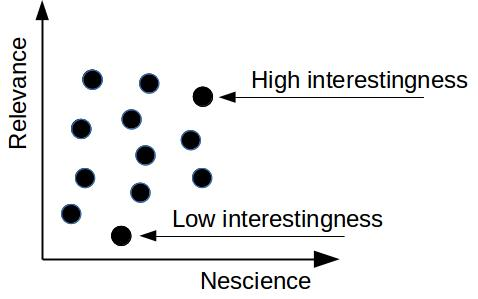
\includegraphics[scale=0.5]{InterestQuestions}
\caption{\label{fig:Interestingness-Questions}Interestingness of Topics}
\end{figure}

\begin{example}
\label{ex:wikipedia-problems}
We can use the collection of Wikipedia articles to identify topics that are interesting as a source of new problems. The starting point of our analysis is the classification contained in the scientific disciplines category of Wikipedia. This category is organized\footnote{Data from November 2014.} into the following main areas: "applied sciences", "behavioral sciences", "cognitive sciences", "formal sciences", "natural sciences", "physical sciences", and "social sciences". In order to evaluate the classification metrics proposed we have used the set of topics corresponding to all pages under any of the subcategories contained in the category "theory of computation" (a subcategory of the category "theoretical computer science", that belongs to the area "formal sciences"). Pages were cleaned up using the same procedure described in Example \ref{ex:diffeq_world}, and the relevance was estimated based on the number of unique visits to each page (please, refer to Chapter \ref{chap:philosophy-science} for more information about this process). Topics that fit our intuitive idea of problem, that is, not very well understood concepts with a high relevance, could include "arithmetical hierarchy" (0.72), "halting problem" (0.65), "floating point" (0.61), "quantum computer" (0.57), and "computable function" (0.55).
\end{example}

The Pythagoras' theorem is not a very interesting research topic by itself, however, it is a very important theorem, since it can be applied to solve many practical problems. A new metric is required to capture this concept of topic that is important because it can be used as a tool to solve other problems. We define the \emph{maturity} of a topic as the inverse of nescience. Intuitively, the more mature a topic is the higher its potential applicability as a tool to solve other open problems, since we know very well how the topic works and how it can be successfully applied. In general, highly immature topics should not be applied to solve open problems, since they could provide wrong answers.

Besides maturity, we also introduce the metric of \emph{applicability} of a topic. Applicability is based on the concept of \emph{applicability graph}. An applicability graph is a directed graph between the research topics (see Figure \ref{fig:ApplicabilityGraph}). An arrow between two topics means that the first topic been successfully applied to explain or solve the second topic. For example, the topic “graph theory” has been applied to the topic “recommendation engines”, since graph theory has been used to solve the problem of which products we should advertise to potential customers on Internet. Given this graph, we define the applicability of a topic as the number of problems to which the topic has been successfully applied. The higher the applicability of a topic, the higher its potential as a tool that can be applied to solve new problems.

\begin{figure}[h]
\centering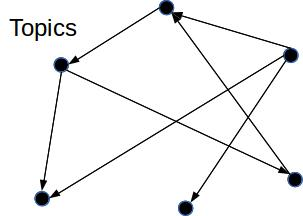
\includegraphics[scale=0.5]{ApplicabilityGraph}
\caption{\label{fig:ApplicabilityGraph}Applicability Graph}
\end{figure}

Finally, we define the concept of interestingness of a topic as a source of interesting tools, that is, how likely is that the topic can be used to solve a new problem, as a function of its maturity and applicability. Intuitively, a topic is interesting as a tool if it has been already applied to many other problems, and it is very well understood topic. For example, the Pythagoras' theorem, although not very relevant as a source of interesting problems, it is very relevant as a source of new applications to other open problems.

\begin{example}
We can use the collection of Wikipedia scientific articles to identify topics with high potential as tools. The procedure used in this example is similar to the one described in Example \ref{ex:wikipedia-problems}, except that the metric applicability has been estimated based in the collection of internal links within Wikipedia itself. The rationale is that if a page is referenced many times by other Wikipedia pages, it is highly likely that it contains useful information. Using this procedure, some examples of topics with high interest as tools in the area of theoretical computer science include "recursion" (0.42), "state space" (0.42), "abstract machine" (0.41), or "ternary numeral system" (0.48).
\end{example}

%
% Section: Interesting questions
%

\section{Interesting Research Questions}
\label{sec:intro_interesting_questions}

Our primary assumption is that a research question is interesting if it meets the following three criteria\index{Criteria for Interesting Questions}:

\bigskip

\begin{description}
\item[C1] The question should be new and original, meaning that it has not been previously considered.
\item[C2] Upon its resolution, there should be a significant increase in our knowledge about one or more specific research topics.
\item[C3] It should have practical applications that could have a substantial (hopefully positive) impact on people's lives.
\end{description}

\bigskip

Some researchers may argue that the requirements presented may not be the most suitable. For instance, researchers from the so-called "hard sciences", such as pure mathematics and theoretical physics, might object that practical applications are not a crucial factor in pursuing an interesting open problem. In such situations, the metrics introduced can be redefined since they are simply mathematical abstractions, and the same methods can still be applied. The methodology described is universal and can be employed in various domains, not only in discovering new research questions. In fact, the metrics and methods outlined can be utilized in any field where there is a vast collection of interconnected describable objects, and the objective is to uncover new and previously unknown objects. The precise definition of concepts like relevance graph, applicability graph, or maturity will be contingent on the field in which the approach is being employed. Nevertheless, as in the case of Chapter \ref{chap:Nescience}, we prefer to present the methodology and new concepts in the specific context of scientific research because it aids in their comprehension.

In the theory of nescience we distinguish two kinds of unknowns, the \emph{known unknown} and the \emph{unknown unknown}. By known unknown we mean all those already known problems for which we do not know their solutions, for example, nobody knows how to cure diabetes, but we know what diabetes is and we are aware that nobody knows how to cure it. By unknown unknown we mean the collection of unknown problems, that is, all those problems that have not been found yet, like for example the Eldermeyer's disease\footnote{We cannot say anything more about the Eldermeyer's disease, since Dra. Eldermeyer will born next year, and it will take her 34 years more to discover the disease named after her.}. The area composed by the unknown unknown problems is a highly interesting one, since it contains those research topics that will be addressed in the future. One of the main goals of this book is to help scientists discover the topics that lay in this unknown unknown area, since that would bring to the present the research problems of the future (see Section \ref{sec:intro_research_topics}). In this section we focus on how to solve the problems of the known unknown area.

An \emph{interesting question} is a ordered pair of topics $t$ and $p$, where $t$ has a high interestingness as tool, and $p$ has high interestingness as problem. Intuitively, the questions would be something like “can we apply the tool described by topic $t$ to solve the problem described by topic $p$?”. The interestingness of the new questions will be measured by means of a function of the interestingness of $t$ and $p$ themselves. In practice what we have to do is to compute all the possible combinations of tools and questions and select those with higher combined interestingness (see Figure \ref{fig:InterestingQuestions}).

\begin{figure}[h]
\centering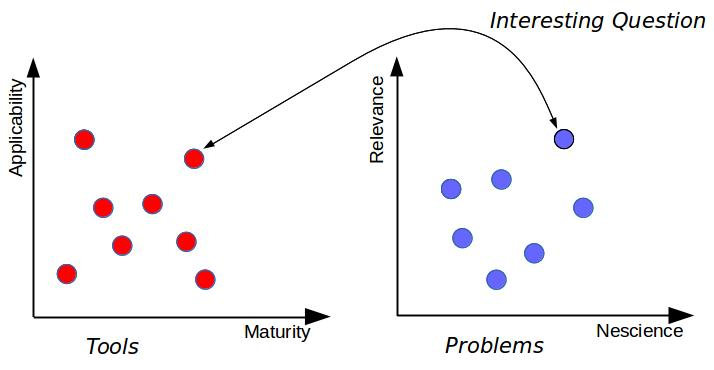
\includegraphics[scale=0.5]{InterestingQuestions}
\caption{\label{fig:InterestingQuestions}Interesting Questions}
\end{figure}

An interesting question is \emph{intradisciplinary} if it combines two topics that are studied in the framework of the same research area (e.g., computer science). An interesting question is \emph{interdisciplinary} if it combines two topics of different research areas (e.g., computer science and philosophy). In principle, the most innovative questions would be interdisciplinary questions, because the probability that somebody has thought about them is lower, since it requires specialists in both research areas working together to come up with that particular question.

\begin{example}
We could combine the topics with high interestingness as tools found in the area of "computer science" with those topics with high interestingness as problems found in the area of "biochemistry" in order to find new interesting interdisciplinary questions. Some examples of the kind of questions we can find with this approach include: “can we use regular expressions to identify DNA genes?” or “can we use a recursive algorithm to characterize proteins tertiary structure?”
\end{example}

Once we have identified an interesting research question, we could use the concept of \emph{conditional model} to see if the tool can help us to understand, or solve, the open problem. A conditional model of a topic $t$ given a perfect model of a second topic $s$ is also a string in the form $\langle TM,a \rangle$, but in this case we require that $TM \left(\langle m_s^\star, a \rangle \right) = t$. That is, the Turin machine $TM$ is able to print $t$ when it has as input both, the incompressible part $a$, and a perfect model $m_s^\star$ for the topic $s$. If the conditional complexity of the open problem given the tool is smaller than its original complexity, then the tool is helpful to solve the problem. The more the tool reduce the length of the conditional model with respect to the original model, the better.

Please note that the methodology presented here is a generic one, in the sense that it can be applied to multiple domains, not only to the discovery of new interesting research questions. The metrics and methods described can be applied to any area where there is a large collection of interrelated describable objects and we are interested in discovering new, previously unconsidered, objects. The exact definition of concepts like relevance graph, applicability graph or maturity will depend on the area in which the methodology is being applied. In Part \ref{part:Applications} of this book, we will describe some examples of other applications, for example, to the identification of new software quality tests.

%
% Applicability
%

\section{Applicability}
\label{sec:applicability}

As mentioned in Example \ref{ex:fixed_point}, the fixed point theorem is not particularly compelling as a research problem on its own. However, it is an essential mathematical result since it has broad applications in proving many other theorems. In this section, we introduce the concept of \emph{applicability}, which is a novel measure enabling us to identify which topics are important since they can serve as as tools for understanding other topics. From a mathematical point of view, we say that a tool can be applied to a topic if the conditional nescience (see Section \ref{sec:conditional_nescience}) of the topic given the tool is smaller that the unconditionall nescience of the topic.

Before to formally define the concept of applicability, first we have to introduce a new bipartite graph that describes which topics has been applied as tools to other topics.

\begin{definition}\index{Applicability graph}
\label{def:applicability-graph}
We define the \emph{applicability graph}, denoted by $AG$, as the directed graph $AG = (\mathcal{T}, E)$, where $\mathcal{T}$ is the set of research topics, and $E\subseteq\left\{ (i,j):i,j\in \mathcal{T} \right\} $. An arc $(i, j)$ belong to $E$ if $N \left( t_i \mid t_j \right) < N \left( t_i \right)$. The weight of the arc $(i, j)$ is given by $w_{ij} = N \left( t_i \right) - N \left( t_i \mid t_j \right)$.
\end{definition}

The applicability graph helps us identify those topics that can be pontentially used as tools to understand other topics. The following defintion formally introduces this idea.

\begin{definition}\index{Applicability}
\label{def:applicability}
Given the applicability graph $AG = (\mathcal{T}, E)$, the \emph{applicability} of a topic $t_i \in \mathcal{T}$, denoted by $A(t_i)$, is defined as the sum of the weights of the arcs in the outdegree of $t_i$, that is:
\[
A(t_i) = \sum_{(i, j) \in E} w_{ij}
\]
where $E$ is the set of arcs in the applicability graph, and $w_{ij}$ is the weight of the arc $(i, j)$.
\end{definition}

A topic with higher applicability will have a greater overall impact on the understanding of other topics, and intuitively, the higher the applicability of a topic, the higher its potential as a tool that can be applied to solve open problems. If a tool has been successfully applied multiple times in the past to address open problems, it is more likely that it can be effectively used to solve other open problems as well.

Next proposition proves that the combination of two topics can only increase their applicability. That is, the more tools we have at our disposal, the more problems we could solve in principle.

\begin{proposition}
Given any two topics $t_1, t_2 \in \mathcal{T}$, we have that $A(t_1) + A(t_2) \geq A(t_1)$.
\end{proposition}
\begin{proof}
Use the same argument than in Proposition \ref{prop:nondecreasing_relevance}.
\end{proof}

In order to better compare the applicability of different topics and understand their relative importance in a standardized way, it is useful to introduce a normalized version of the applicability measure.

\begin{definition}\index{Normalized Aapplicability}
\label{def:normalized-applicability}
Given the applicability graph $AG = (\mathcal{T}, E)$, the \emph{normalized applicability} of a topic $t_i \in \mathcal{T}$, denoted by $A_n(t_i)$, is defined as the ratio of the applicability of $t_i$ to the maximum possible applicability value, expressed as:
\[
\tilde{A}(t_i) = \frac{A(t_i)}{\max_{t_k \in \mathcal{T}} A(t_k)}
\]
where $A(t_i)$ is the applicability of topic $t_i$ as defined in Definition \ref{def:applicability}, and $\max_{t_k \in \mathcal{T}} A(t_k)$ is the maximum applicability value among all topics in $\mathcal{T}$.
\end{definition}

Normalized applicability scales the original applicability value of a topic to a range between 0 and 1, allowing for easier comparison across different topics.

In practice, it is very difficult to compute the applicability graph, since for the majority of the topics, the quantity $N \left( t_i \mid t_j \right)$ has not been estimated. In order to solve this problem, we can use an approximation to the applicabilitiy graph, in which the arcs have no weight, and an edge $(i, j)$ represents that the topic $j$ has been applied to solve the problem $i$. For example, there would be a direct link between the topics "graph theory" and "recommendation engines", since graph theory has been successfully applied to the problem of how to recommend purchase items to customers over Internet.

\begin{definition}\index{Simplified applicability graph}
\label{def:simplified-applicability-graph}
We define the \emph{simplifiled applicability graph}, denoted by $SAG$, as the directed graph $SAG = (\mathcal{T}, E)$, where $\mathcal{T}$ is the set of research topics, and $E\subseteq\left\{ (i,j):i,j\in \mathcal{T} \right\} $. An arc $(i, j)$ belong to $E$ if the topic $j$ has been used to understand topic $i$.
\end{definition}

Using this simplified version of the applicability graph, the concept of applicability becomes:

\begin{definition}\index{Simplified applicability}
\label{def:simplified-applicability}
We define the \emph{simplified applicability} of a topic $t\in \mathcal{T}$, denoted by $SA(t)$, as the outdegree of that node in the applicability graph, that is:
\[
SA(t) = outdeg(t)
\]
\end{definition}

And the corresponding normalized version becomes:

\begin{definition}\index{Normalized simplified applicability}
\label{def:normalized-simplified-applicability}
Given the simplified applicability graph $SAG = (\mathcal{T}, E)$, the \emph{simplified normalized applicability} of a topic $t_i \in \mathcal{T}$, denoted by $SA_n(t_i)$, is defined as the ratio of the simplified applicability of $t_i$ to the maximum possible simplified applicability value, expressed as:
\[
SA_n(t_i) = \frac{SA(t_i)}{\max_{t_k \in \mathcal{T}} SA(t_k)}
\]
where $SA(t_i)$ is the simplified applicability of topic $t_i$ as defined in Definition \ref{def:applicability}, and $\max_{t_k \in \mathcal{T}} SA(t_k)$ is the maximum applicability value among all topics in $\mathcal{T}$.
\end{definition}

When using topics as tools, we are primarily interested in those topics that are better understood. Generally, relying on a background knowledge that is poorly understood is not advisable, even if it significantly reduces the (conditional) nescience of our problem. In the following definition, we will introduce the concept of the maturity of a topic as one minus its nescience.

\begin{definition}\index{Maturity}
Given a topic $t \in \mathcal{T}$, we define the \emph{maturity} of topic $t$, denoted as $M(t)$, as:
\[
M(t) = \nu(t)^{-1}
\]
\end{definition}

Intuitively, the more mature a topic is, the greater its utility in solving other open problems. Highly immature topics should not be applied as tools to address open problems, as doing so would merely transfer our lack of understanding from one topic to another.

\begin{example}
Linear regression is a highly mature topic, since its nescience is very small.
\end{example}

Finally, we define the concept of interestingness of a topic as a source of interesting tools, that is, how likely is that the topic can be used to solve a new problem, as a function of its maturity and applicability. Similar to the definition of relevance introduced in the previous section, topics can be visualized within a two-dimensional vector space, where one dimension represents maturity and the other represents applicability. The interestingness of a topic will be determined by its Euclidean distance from the origin.

\begin{definition}\index{Interestingness of a topic as a tool}
Given a topic $t \in \mathcal{T}$, we define the \emph{interestingness of the topic as a tool}, denoted by $IT(t)$, as:
\[
IT(t) = \sqrt{ M(t)^2 +  A(t)^2 }
\]
\end{definition}

Intuitively, a topic is considered interesting as a tool if it is thoroughly understood and has already been applied to numerous other problems.

\begin{example}
The Pythagorean theorem (in a right-angled triangle, the square of the length of the hypotenuse is equal to the sum of the squares of the other two sides) is undoubtedly one of the most widely used and applied theorems in various fields and practical situations, including but not limited to: engineering (calculating distances, angles, and forces in structures and mechanical systems), architecture (determining lengths and angles in building design and construction projects), land surveying (measuring distances and calculating areas of land parcels), physics (analyzing problems in mechanics, optics, and electromagnetism), computer graphics and game development (calculating distances and angles in 2D and 3D spaces) or trigonometry(serving as a foundation for the study of trigonometric functions and their applications). The widespread application of the Pythagorean theorem to so many fields is due to its simplicity and its ability to describe complex geometric relationships.
\end{example}


%
% Section: Interesting Questions
%

\section{Interesting Questions}

In the quest to uncover novel research questions, combining existing topics from various fields can yield fascinating results. By applying tools and methodologies from one topic to solve problems in another, researchers can explore innovative avenues and potentially make groundbreaking discoveries. In the following section, we delve into the methodology of combining topics to generate questions, along with the concept of interestingness and interdisciplinary research.

In our methdology, a interesting question emerges from the combination of two pre-existing topics. Given a pair of a topics in $t_1, t_2 \in \mathcal{T}$, the question can be framed as "\emph{can we apply the tool described by topic $t_1$ to solve the problem described by topic $t_2$?}".

\begin{definition}\index{Question}
Given two topics $t_1, t_2 \in \mathcal{T}$, a \emph{question}, denoted by $Q_{t_1 \rightarrow t_2}$, is the ordered pair $\left(t_1, t_2\right)$.
\end{definition}

The most intriguing questions emerge when topic $t_1$ exhibits high interestingness as a tool, and topic $t_2$ demonstrates high interestingness as a problem. We define the interestingness of a question using the Euclidean distance, taking into account the interestingness of topics $t_1$ and $t_2$ as points in a two-dimensional space, with coordinates $(A_{t_1}, M_{t_1})$ and $(R_{t_2}, N_{t_2})$, respectively. The coordinates of the resulting vector represent the interestingness of a question with $t_1$ as a tool and $t_2$ as a problem.

\begin{definition}\index{Interestingness of a question}
Let $t_1$ and $t_2 \in \mathcal{T}$ be two topics. The \emph{interestingness} of the question $Q_{t_1 \rightarrow t_2}$, denoted by $IQ_{t_1 \rightarrow t_2}$, is given by:
\[
IQ_{t_1 \rightarrow t_2} = \sqrt{ (A_{t_1} + R_{t_2})^2 + (M_{t_1} + N_{t_2})^2 }
\]
\end{definition}

Employing the Euclidean distance in this way enables a geometric interpretation of the interestingness of a question based on the vector representation of topics in the interestingness space. The larger the magnitude of the vector representation, the higher the interestingness of the resulting question.

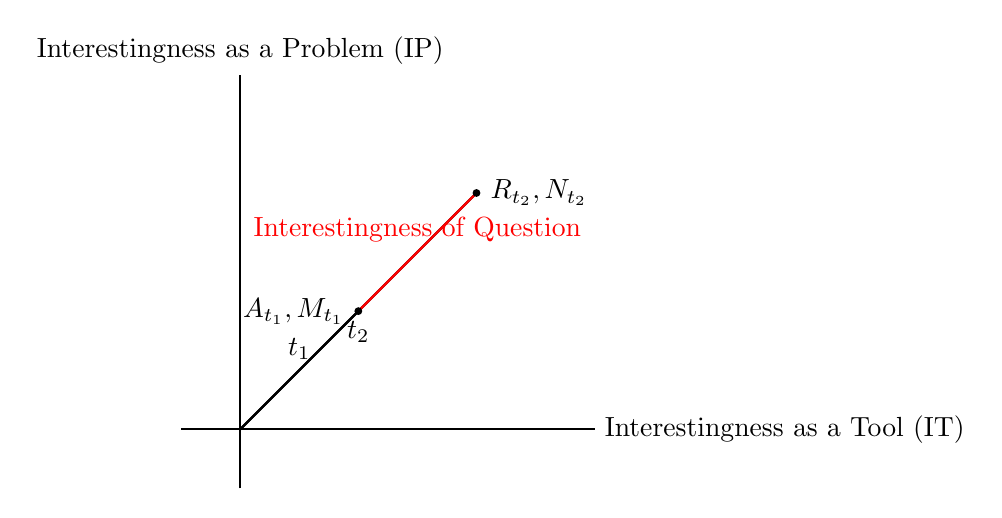
\begin{tikzpicture}[
    scale=1.5,
%    axis/.style={thick, ->, -latex', >=Stealth},
    axis/.style={thick},
%   vector/.style={thick, ->, -latex', >=Stealth, color=blue},
    vector/.style={thick},
    point/.style={circle, inner sep=1pt, fill, color=black}
]

% Coordinate axes
\draw[axis] (-0.5, 0) -- (3, 0) node[right] {Interestingness as a Tool (IT)};
\draw[axis] (0, -0.5) -- (0, 3) node[above] {Interestingness as a Problem (IP)};

% Points for t1 and t2
\coordinate (t1) at (1, 1);
\coordinate (t2) at (2, 2);

% Vectors for t1, t2, and the sum
\draw[vector] (0, 0) -- node[pos=0.5, above] {$t_1$} (t1);
\draw[vector] (0, 0) -- node[pos=0.5, below] {$t_2$} (t2);
\draw[vector, color=red] (t1) -- node[pos=0.5, above] {Interestingness of Question} (t2);

% Points and labels for t1 and t2
\node[point, label={left:$A_{t_1}, M_{t_1}$}] at (t1) {};
\node[point, label={right:$R_{t_2}, N_{t_2}$}] at (t2) {};

\end{tikzpicture}

In practice, we must calculate all possible combinations of topics with high interestingness as tools and those with high interestingness as problems. We then select the combinations with the highest interestingness as questions. Naturally, most questions generated using this approach will be meaningless, much like those arising during brainstorming sessions when researchers attempt to identify new tools for tackling difficult problems.

This methodology can be applied in other scenarios as well. For instance, a researcher familiar with problem $p$ might be interested in finding applicable tools to solve it. Similarly, a researcher specializing in tool $t$ may be interested in discovering open problems where his expertise can be applied.

The above procedure can be easily generalized to encompass multiple tools and possibly multiple problems. This leads to the application of two tools to a given problem ($ t_1 + t_2 \rightarrow p$), the application of a single tool to the combination of two problems ($t \rightarrow p_1 + p_2$), and so on. The exact meaning of these tool and problem combinations depends on the topics themselves and is left to the researcher's creative interpretation.

At times, it is beneficial to limit our search to specific areas of knowledge to identify interesting questions.

\begin{definition}\index{Intradisciplinary question} \index{Interdisciplinary question}
Let $\mathcal{A} \subset \mathcal{T}$ be a research area, and $t_1, t_2 \in \mathcal{T}$ be two topics. If both topics belongs to the same area, meaning $t_1, t_2 \in \mathcal{A}$, we say that the question $Q_{t_1 \rightarrow t_2}$ is \emph{intradisciplinary}, otherwise, we say that the question is \emph{interdisciplinary}.
\end{definition}

The most innovative questions tend to be interdisciplinary, as they have a lower likelihood of having been considered previously. This is because they require collaboration between specialists from different research areas. Interdisciplinary questions address our requirement \textbf{C1} for interesting questions, which dictates that the question must be new and original.

%
% Section: New Research Topics
%

\section{New Research Topics}
\label{sec:New_Research_Topics}

{\color{red} TODO: Review this section}

In the previous section our focus was in how to find new interesting research questions. In this section we will go one step beyond, and we will show how to identify new, previously unknown, research topics.

\begin{definition}\index{Unknown frontier}
In the two-dimensional space defined by relevance and nescience, the \textit{unknown frontier}, denoted by $\mathbb{F}$, is defined as the following arc:
\[
\mathbb{F} = \left\{(x,y) \mid x^{2}+y^{2}=max(\{N^2_{t} + R^2_{t}, t \in T'\}),x>0,y>0\right\} 
\]
\end{definition}

If we plot all the known research topics according to their relevance and nescience, the unknown frontier will cover them. Intuitively the \emph{unknown frontier} marks the frontier between what we do not know and we are aware that we do not know (we do not fully understand those topics), and what we do not known and we are not yet aware that we do not known those topics. This intuitive property is in general terms, since it may happen that some unknown topics lie under the unknown frontier as well.

\begin{definition}\index{New topics area}
Lets $T'$ the set of known research topics. The \emph{new topics area}, denoted by $\mathbb{S}$, is defined by:
\[
\mathbb{S} = \left\{(x,y) \mid x^{2}+y^{2}>max(\{N^2_{t} + R^2_{t}, t \in T'\}),x>0,y>0\right\} 
\]
\end{definition}

The new topics area contains all those unknown topics that we are not aware we do not know them (unknown unknown). The big issue is how to reach this new topics area if we do not know anything about the topics included in that area.

\begin{proposition}
\label{prop:new-topics-area}
Let $r \in T$ be a topic, if  $N^2_{r} + R^2_{r} > max(\{N^2_{t} + R^2_{t}, t \in T'\}$ then $t \in T \setminus T'$.
\end{proposition}
\begin{proof}
Let $N^2_{r} + R^2_{r} > max(\{N^2_{t} + R^2_{t}, t \in T'\}$ and suppose that $r \in T'$, then have that $max(\{N^2_{t} + R^2_{t}, t \in T'\}) \geq N^2_{r} + R^2_{r}$ that it is a contradiction, and so $t \in T \setminus T'$.
\end{proof}

Proposition \ref{prop:new-topics-area} together with the fact that the combined nescience of two topics is higher than the nescience of any of them isolated (Proposition {\color{red} XXX}), and that their combined relevance is higher that the relevance of any of them (Proposition \ref{prop:nondecreasing_relevance}), a possible approach to identify new topics could be by means of combining already existing interesting problems. In Figure \ref{fig:New-Topics} is depicted graphically the idea.

\begin{figure}[h]
\centering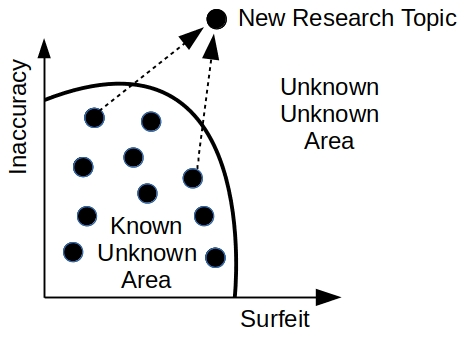
\includegraphics[scale=0.4]{NewTopics}
\caption{\label{fig:New-Topics}The discovery of new research topics}
\end{figure}

\begin{definition}\index{New topic}
Given two topics $t_{1}, t_{2} \in T'$, a \emph{new topic}, denoted by $S_{\left\{ t_{1},t_{2}\right\}}$, is the unordered pair $\left\{ t_{1},t_{2}\right\}$.
\end{definition}

The exact meaning of the new topic that results as the combination of topics $t_{1}$ and $t_{2}$ is left to the creative interpretation of the researcher.

\begin{definition}\index{Interestingness of a new topic}
The \emph{interestingness} of the new topic, denoted by $IS_{\left\{ t_{1},t_{2}\right\} }$, is given by:
\[
IS_{\left\{ t_{1},t_{2}\right\} } = R_{t_{1}}R_{t_{2}}+N_{t_{1}}N_{t_{2}}
\]
\end{definition}

In practice, what we have to do is to compute all possible combination of those topics with very large interestingness as problems $IP_{t}$ with themselves, and select the combinations with higher $IS$. Of course, some of the combinations generated would be totally meaningless. Advanced techniques from the area of natural language processing or machine learning could be used to try filter out those nonsense combinations.

\begin{definition}\index{Intradisciplinary new topic} \index{Interdisciplinary new topic}
Let $A \subset T$ a research area, and $t_{1}, t_{2} \in T$ two topics. If both topics belongs to the same area, that is $t_{1}, t_{2} \in A$, we say that the new topic $S_{\left\{ t_{1},t_{2}\right\} }$ is \emph{intradisciplinary}, otherwise, we say that the topic is \emph{interdisciplinary}.
\end{definition}

Again, the most innovative new topics would be by the combination of interdisciplinary topics, because the probability that somebody has already though about them is lower.

%
% Section: Classification of Research Areas
%

\section{Classification of Research Areas}

In the same way we studied the nescience of research areas (see Section \ref{sec:nescience_areas}), we could also study the interestingness of research areas.

\begin{definition}\index{Average interestingness of an area}
Given a research area $A\subset T$, we define the \emph{average interestingness
of the area as a source of interesting tools} by
\[
IT_{A}=\frac{1}{n}\sum_{t\in A}IT_{t}
\]
and the \emph{average interestingness of the area as a source of interesting
problems} by
\[
IP_{A}=\frac{1}{n}\sum_{t\in A}IP_{t}
\]
where $n$ is the cardinality of $A$.
\end{definition}

In this way we could compute the interestingness of mathematics, physics, biology, social sciences, and other disciplines as a source of interesting tools and problems. Other alternative measures of centrality and dispersion could be used for the characterization of research areas as well.

As I will show in Chapter \ref{chap:The-Scientific-Method}, the interestingness of mathematics as a source of tools is higher than the interest of social sciences, since mathematics is composed of topics with a high applicability that are very well understood, and that is not the case, in general, for social sciences. On the other hand, the interestingness of social sciences as a source of problems is higher than the interest of mathematics, since the topics studied by the social sciences are more relevant to humankind \footnote{Please mind that I am not saying that the topics addressed by mathematics are not relevant to humankind, what I am saying is that, in relative terms, the problems addressed by social sciences have a higher relevance.} and, in general, not very well understood.

\begin{example}\index{Areas in decay}
We could use the interestingness of an area to identify research areas in decay. A knowledge area is in decay (from the research point of view) if it has no enough interesting research problems. For example, although the aerodynamics of zeppelins is not fully understood (still some nescience), it is not longer useful (low relevance), since people does not use zeppelins to travel anymore, and so, the average interestingness is very low. Another example of area in decay is classical geometry: although it is relevant, our understanding of this subject is nearly perfect, since there are almost no unsolved problems, and so, its average nescience is very low. However, on the contrary to what happens in case of the aerodynamics of zeppelins, classical geometry is still very interesting as a source of tools.
\end{example}

It is worth to mention that we could add other metrics to provide a finer, or even alternative, characterization of the unknown unknown area. For example, we could add to nescience and relevance a third dimension with the probability that a topic description is true. However, these extended or alternative characterizations will be not considered in this book. Fortunately, the idea of how to reach the unknown unknown area is the same, regardless of the number and the metrics used (as long as these metrics satisfy some minimal mathematical properties, described in Chapters \ref{chap:Nescience} and \ref{chap:Interesting-Research-Questions}).

%
% References
%

\section*{References}

Popper and falsificationism

{\color{red} Review the following references}

\begin{itemize}

\item Freitas, A. A. (1999). On Objective Measures of Rule Surprisingness. In Proceedings of the Second European Symposium on Principles of Data Mining and Knowledge Discovery (PKDD '98), pp. 1-9.

\item Gureckis, T. M., \& Goldstone, R. L. (2009). How You Named Your Child: Understanding The Relationship Between Individual Decision Making and Collective Outcomes. Topics in Cognitive Science, 1(4), 651-674.

\item Klein, J. T. (1990). Interdisciplinarity: History, Theory, and Practice. Wayne State University Press.

\item Kuhn, T. S. (1962). The Structure of Scientific Revolutions. University of Chicago Press.

\item Newell, A., \& Simon, H. A. (1972). Human Problem Solving. Prentice-Hall.

\item Page, S. E. (2007). The Difference: How the Power of Diversity Creates Better Groups, Firms, Schools, and Societies. Princeton University Press.

\item Rescher, N. (1986). The Riddle of Existence: An Essay in Idealistic Metaphysics. University Press of America.

\item Schelling, T. C. (1978). Micromotives and Macrobehavior. W. W. Norton \& Company.

\end{itemize}
